\lstset{language=C++}
\section{EMPASS: a parallel ABM simulator}
This Chapter contains an introduction to parallel computing and explains
why it is important to adopt a parallel approach to ABM with the recent
boom in the market of parallel CPU\nomenclature{CPU}{Central Processing Unit}
and GPU\nomenclature{GPU}{Graphical Processing Unit}.
The approach used in this Thesis was to implement a parallel ABM engine to speed
 up the simulations by using a software framework called OpenMP which lets the user
exploit the recent multi core processors from Intel or similar.
\subsection{Traditional computing paradigm}
Traditionally, software has been written for serial computation to be run on
a single computer having a single Central Processing Unit (CPU).
A problem is solved by an algorithm described by a discrete series of instructions,
 which are executed one after another - see Figure \ref{Fig:Parallel:serialProblem}.
The bottleneck is that only one instruction may execute at any moment in time
 and is radicated in the original Von Neumann architecture -see Figure \ref{Fig:Parallel:Neumann}
that was designed in the 1945.
The control unit fetches instructions or data from memory, decodes the instructions
and then sequentially coordinates operations to accomplish the programmed task.

\begin{figure}[htbp]
\begin{center}
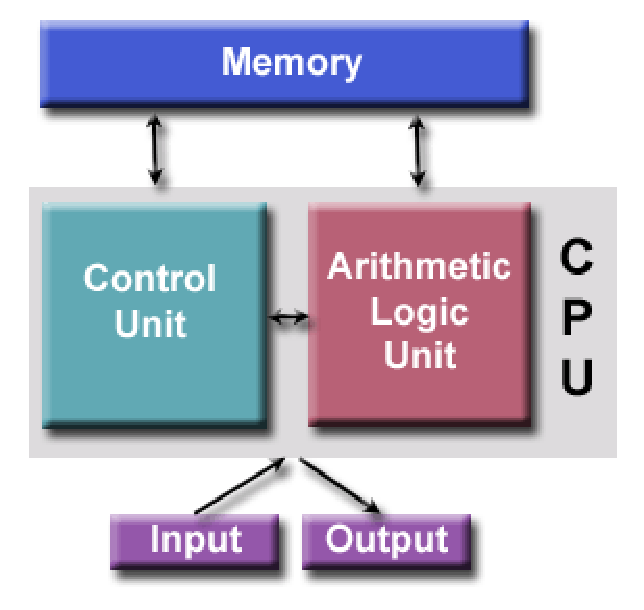
\includegraphics[width=0.5 \textwidth ]{OpenMP/vonNeumann.eps}
\end{center}
\small{
\caption[Von Neumann architecture]{
The von Neumann architecture is based on 4 components:
the memory, the control unit, the arithmetic logic unit and
an input and output channel.
\label{Fig:Parallel:Neumann}}}
\end{figure}

\begin{figure}[htbp]
\begin{center}
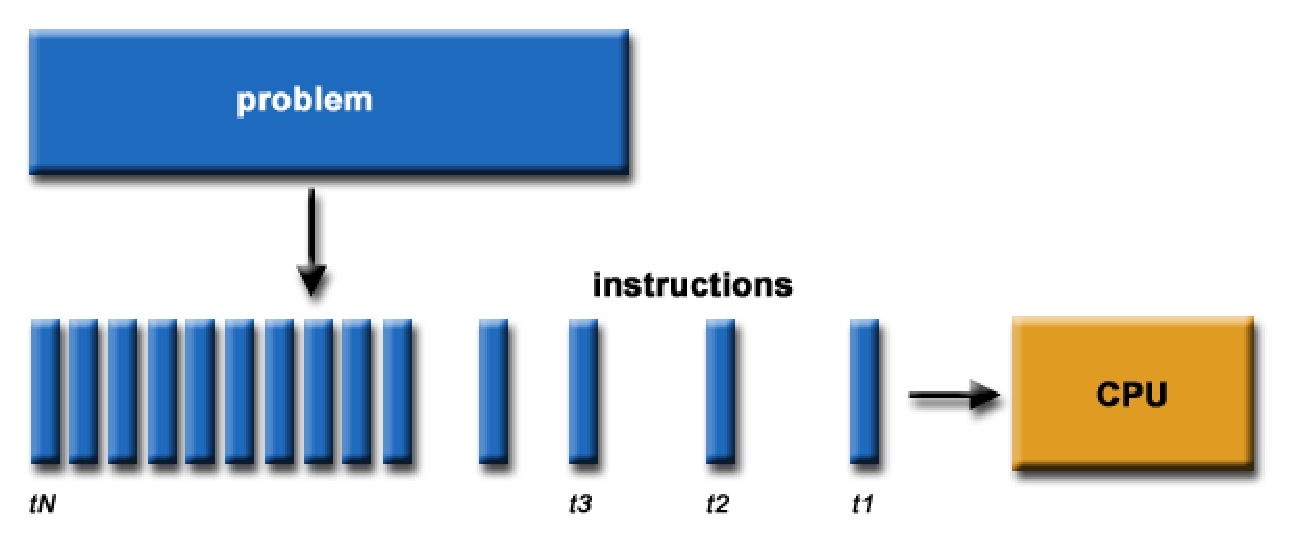
\includegraphics[width=0.8 \textwidth ]{OpenMP/serialProblem.eps}
\end{center}
\small{
\caption[Serial Problem computation]{
The problem is divided in a set of instructions which are executed
at sequential time steps.
\label{Fig:Parallel:serialProblem}}}
\end{figure}

Parallel computing adopts a new architecture to bypass the bottleneck of
serial execution.

\subsection{Parallel computing paradigm}
Parallel computing is the simultaneous use of multiple computing resources
to solve a computational problem.
To avoid serial execution the algorithm is executed on multiple CPUs.
To do so the problem must be broken into discrete parts that can be
 solved concurrently like in Figure \ref{Fig:Parallel:parallelProblem} .
Each part is further broken down to a series of instructions which are executed
simultaneously on different CPUs.

\begin{figure}[htbp]
\begin{center}
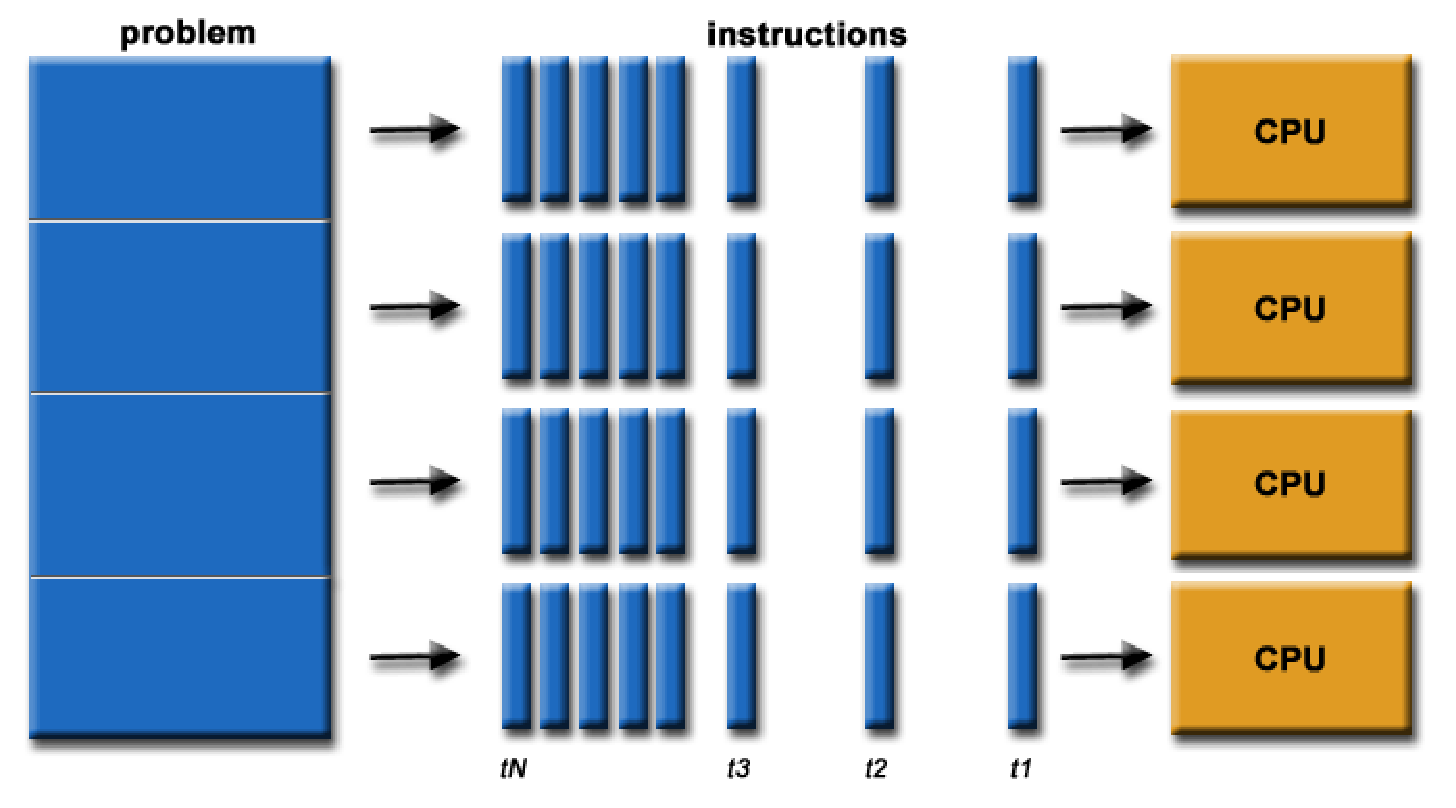
\includegraphics[width=0.8 \textwidth ]{OpenMP/parallelProblem.eps}
\end{center}
\small{
\caption[Serial Problem computation]{
The problem is divided into blocks which are then divided in a set of instructions
allocated to different CPUS.
\label{Fig:Parallel:parallelProblem}}}
\end{figure}

The distribution of the computational load can be achieved by:
\begin{itemize}
\item  A single computer with multiple processors
\item  A computer network
\item  A combination of both
\end{itemize}

The problem needs to fulfil the basic property
\begin{itemize}
\item  Broken apart into discrete pieces of work that can be solved simultaneously;
\item Execute multiple program instructions at any moment in time;
\item Solved in less time with multiple compute resources than with a single compute resource.
\end{itemize}

\subsection{Flynn's Classical Taxonomy}
Flynn's Taxonomy was introduced in 1966 to rationalise and classify the
different type of parallel hardware architectures.
The taxonomy contains 4 categories:
\begin{itemize}
\item Single Instruction Single Data: the CPU executes a single stream of
instructions on a single stream of data like in Figure \ref{fig:Parallel:SISD}
\item Single Instruction Multiple Data: each CPU executes the same stream of
instructions on different streams of data like in Figure \ref{fig:Parallel:SIMD}
\item Multiple Instruction Single Data: each CPU executes different
streams of instructions on the same stream of data like in Figure \ref{fig:Parallel:MISD}
\item Multiple Instructions Multiple Data: each CPU executes different
streams of instructions on the same stream of data like in Figure \ref{fig:Parallel:MIMD}
\end{itemize}

\begin{figure}[htbp]
  \begin{center}
      \subfigure[SISD diagram]{
	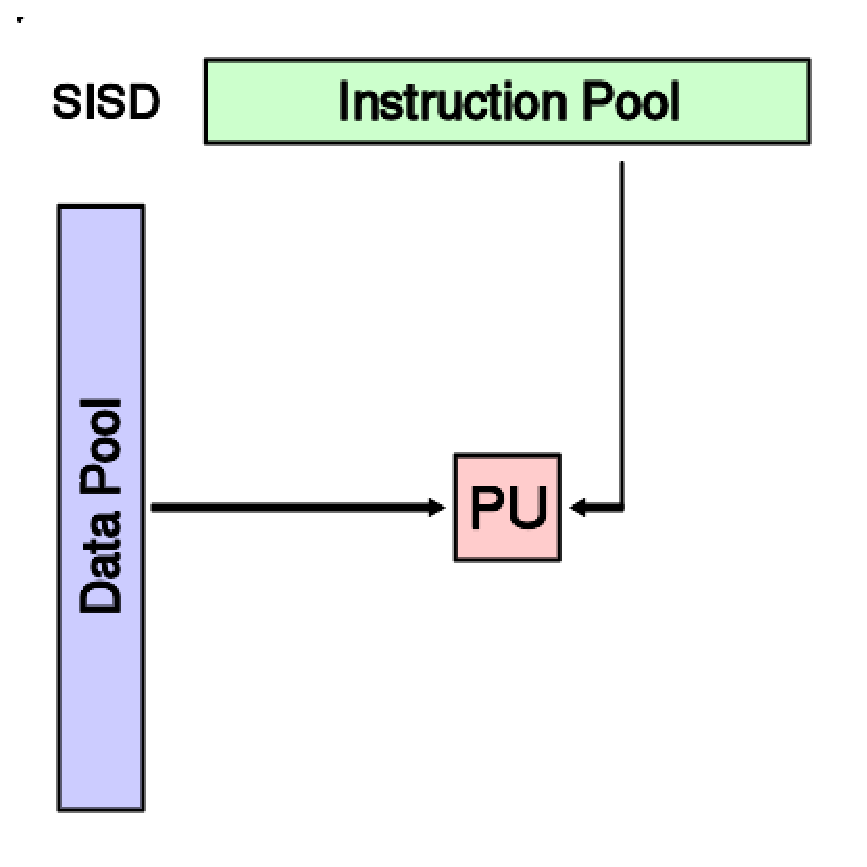
\includegraphics[width=0.4 \textwidth]{figures/OpenMP/SISD_diagram.eps}}
      \hspace{1pt}
      \subfigure[SISD program]{
	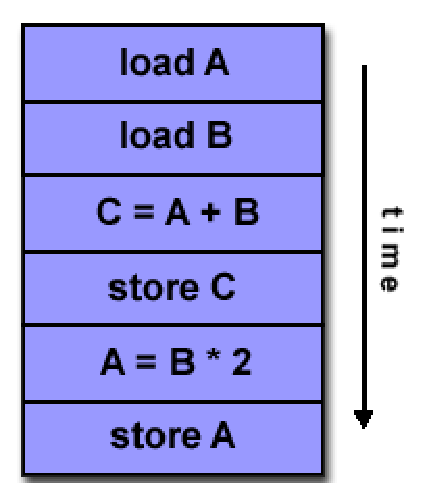
\includegraphics[width=0.3 \textwidth]{figures/OpenMP/SISD_program.eps}}
    \caption[SISD architecture]{ \label{fig:Parallel:SISD}}
  \end{center}
\end{figure}

\begin{figure}[htbp]
  \begin{center}
      \subfigure[SISD diagram]{
	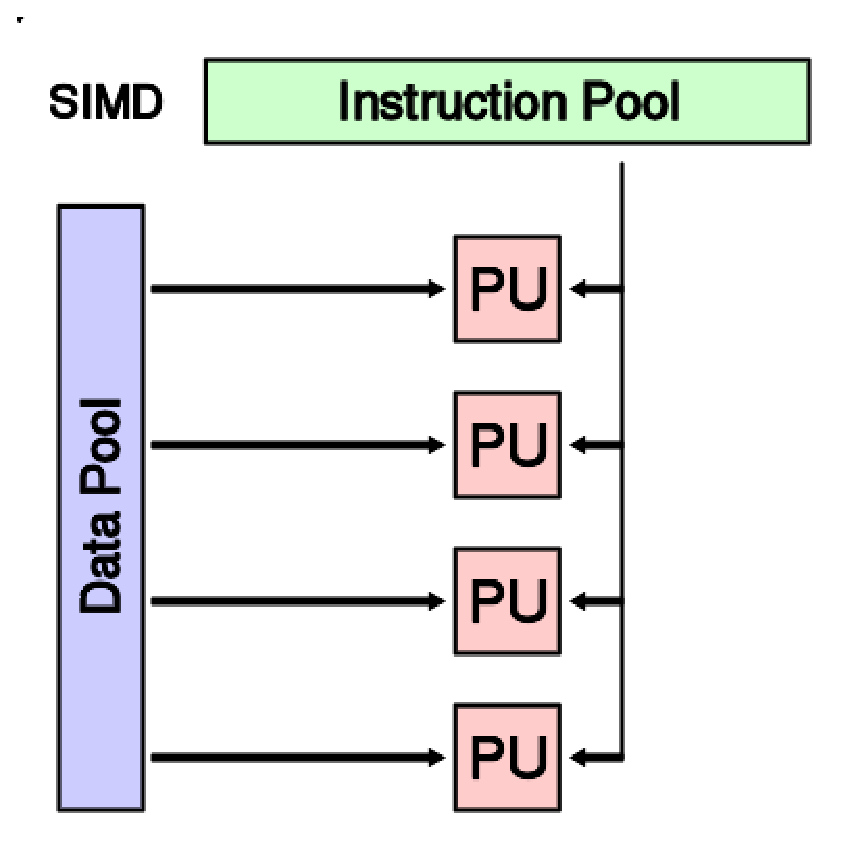
\includegraphics[width=0.4 \textwidth]{figures/OpenMP/SIMD_diagram.eps}}
      \hspace{1pt}
      \subfigure[SISD program]{
	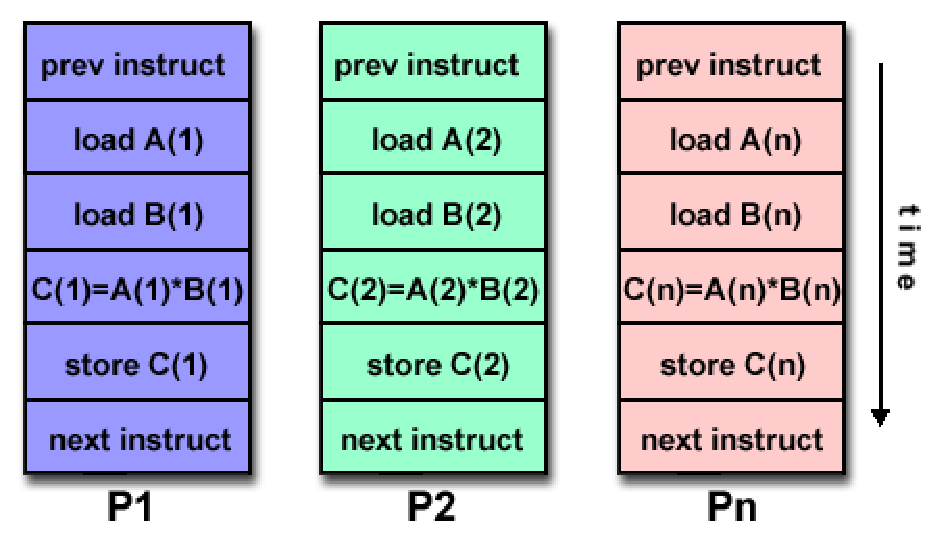
\includegraphics[width=0.4 \textwidth]{figures/OpenMP/SIMD_program.eps}}
    \caption[SIMD architecture]{ \label{fig:Parallel:SIMD}}
  \end{center}
\end{figure}

\begin{figure}[htbp]
  \begin{center}
      \subfigure[SISD diagram]{
	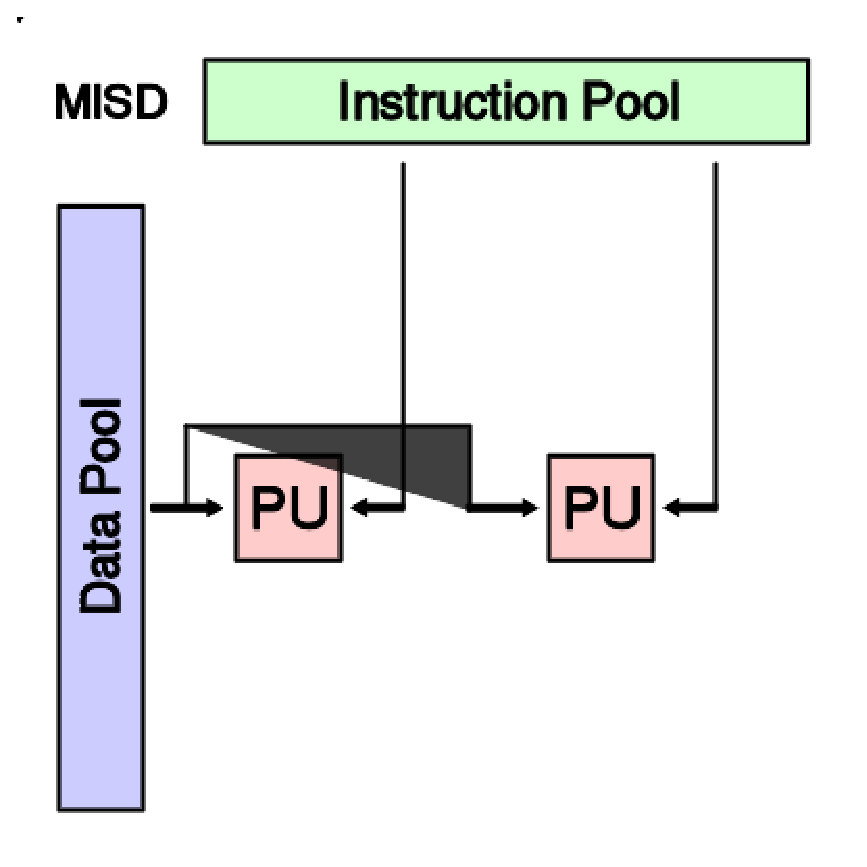
\includegraphics[width=0.4 \textwidth]{figures/OpenMP/MISD_diagram.eps}}
      \hspace{1pt}
      \subfigure[SISD program]{
	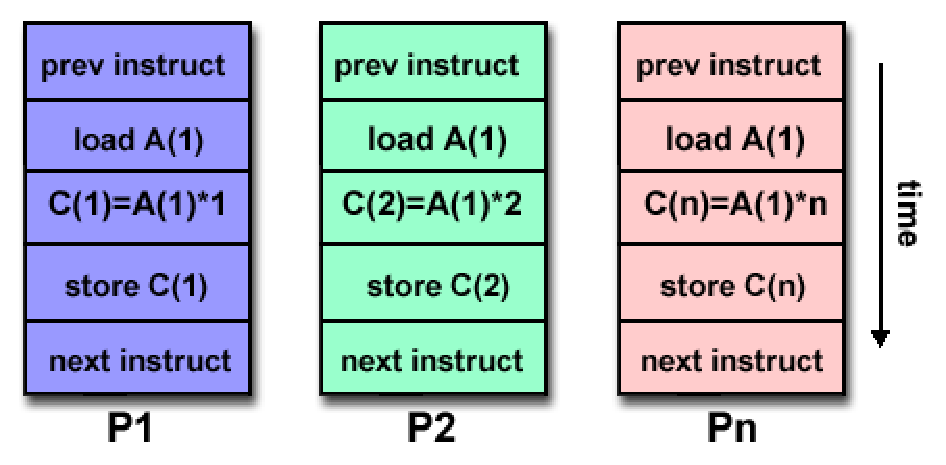
\includegraphics[width=0.4 \textwidth]{figures/OpenMP/MISD_program.eps}}
    \caption[MISD architecture]{ \label{fig:Parallel:MISD}}
  \end{center}
\end{figure}

\begin{figure}[htbp]
  \begin{center}
      \subfigure[SISD diagram]{
	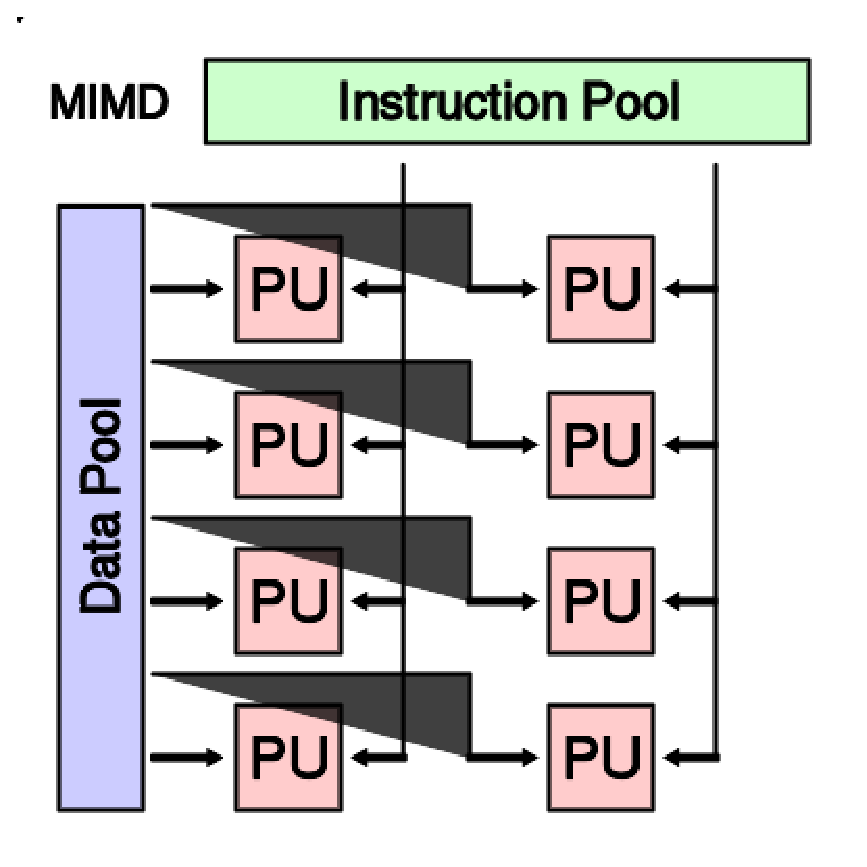
\includegraphics[width=0.4 \textwidth]{figures/OpenMP/MIMD_diagram.eps}}
      \hspace{1pt}
      \subfigure[SISD program]{
	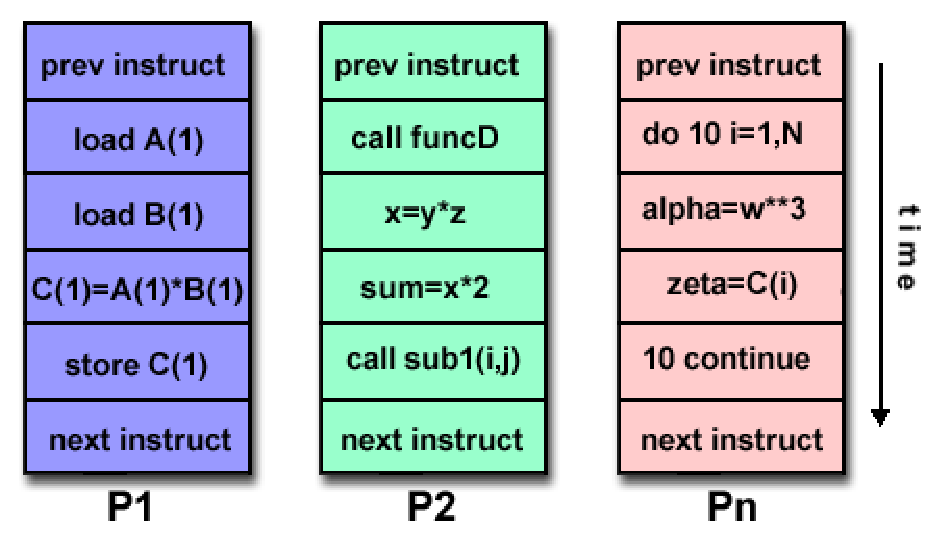
\includegraphics[width=0.4 \textwidth]{figures/OpenMP/MIMD_program.eps}}
    \caption[SISD architecture]{ \label{fig:Parallel:MIMD}}
  \end{center}
\end{figure}

On top of this hardware layer, it was necessary to define a set of parallel
programming models.
The most common ones used are:
\begin{itemize}
 \item Shared Memory
 \item Threads
 \item Message Passing
 \item Data Parallel
 \item Hybrid
\end{itemize}
Those models are not dependent on any particular machine or memory architecture.
There is no absolute best nor absolute worse, but surely there are
better implementations or open source solutions.

\begin{figure}[htbp]
\begin{center}
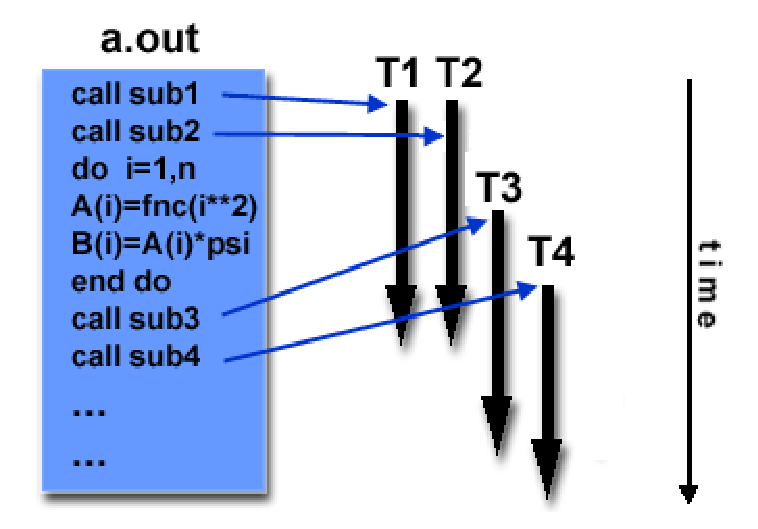
\includegraphics[width=0.8 \textwidth ]{OpenMP/thread_model.eps}
\end{center}
\small{
\caption[The Thread model]{
In the Thread Model a sequential program a.out can be executed as several threads
T1,T2,T3,T4 which executes concurrently the sub routines of the program.
\label{Fig:Parallel:threadModel}}}
\end{figure}

One of the most successful model in the consumer level entry is is the
Thread model, which is adopted both
by Unix and Microsoft operative systems.
In the threads model of parallel programming, a single process can have
 multiple, concurrent execution paths as in the Figure \ref{Fig:Parallel:threadModel}.

Threads are commonly associated with shared memory architectures
and operating systems.
The UNIX standard is POSIX and OpenMP.
\subsection{Open MP}
OpenMP stands for Open Multi-Processing but the original acronym was
Open specifications for Multi-Processing via collaborative work between
interested parties from the hardware and software industry, government and academia.

\begin{figure}[htbp]
\begin{center}
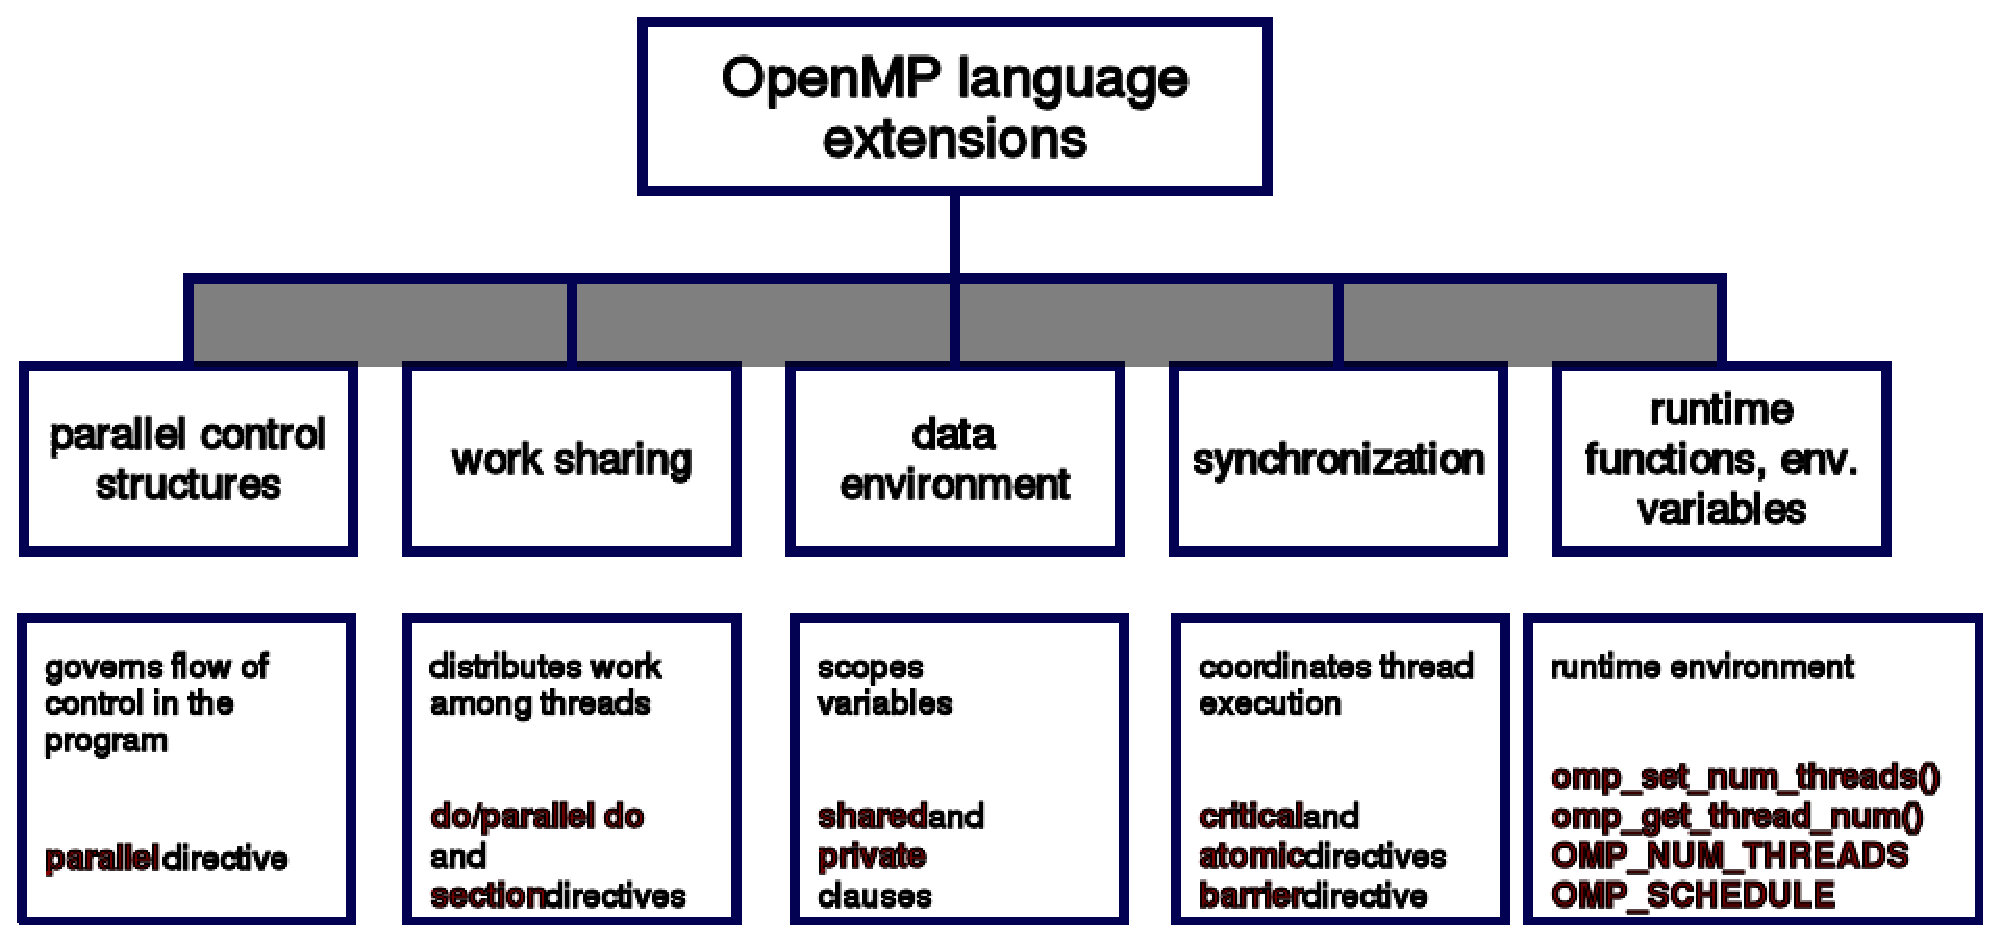
\includegraphics[width=0.8 \textwidth ]{OpenMP/language_extensions.eps}
\end{center}
\small{
\caption[OpenMP language]{
OpenMP language structure: a set of pragma directives and keywords.
\label{Fig:Parallel:language}}}
\end{figure}

OpenMP is an application program Interface (API) that may be used to explicitly
 direct multi-threaded, shared memory parallelism.
It is comprised of three primary API components (see Figure \ref{Fig:Parallel:language}):
\begin{itemize}
\item Compiler Directives
\item Runtime Library Routines
\item Environment Variables
\end{itemize}
Open MP is Portable because the API is specified for $C/C++,Fortran$ and
most major platforms have been implemented including Unix/Linux platforms and Windows NT
Open MP is standardised and endorsed by a group of major computer hardware
and software vendors
The following table \ref{tab:Parallel:comparison} compares the POSIX with
the OpenMP standard.


\begin{table}[htbp]
\centering
\begin{tabular}{| c| p{3.5 cm} | p{3.5 cm} |}
\hline
Standard & Posix & OpenMP \\
\hline
Language supported & C only & $C,C++$ and Fortran\\
\hline
Programming API & Library based requires parallel coding & Compiler directive based \\
\hline
Usability & Requires complex explicit coding & Easy and simple to use, incremental parallelism \\
\hline
Standard & IEEE POSIX 1003.1c standard (1995) & The OpenMP Fortran API was released October 28, 1997. The C/C++ API was released in late 1998.  \\
\hline
\end{tabular}
\caption[Posix vs OpenMP standard]{Table comparing the two most common standards}
\label{tab:Parallel:comparison}
\end{table}

The author decided to use OpenMP for implementing parallelism in the simulator
because it is the most convenient choice in terms of language support and
implementation.
\subsection{ABM simulation engine with OpenMp}
The author developed an ABM engine called ``Multi Parallel Agent'' with codename
``Empass'' which is a minimalist particle engine written in $C \setminus C++$.
The scope of this software project is to use OpenMP and thus have a fully
portable parallel implementation.
The motivation for developing a new simulator is that existing softwares did not
do well in terms of language support, flexibility and scalability.
The most popular engines for multi agent robot simulations are:

\begin{itemize}
\item RePast: A popular Java-based social complexity simulation toolkit.
\item Ascape: Another popular Java-based social complexity simulation toolkit.
\item Swarm: the venerable Objective-C and TCL-based social complexity simulator,
      from which RePast and Ascape (and MASON) owe much.
\item TeamBots: A Java-based high-level, 2D abstract robotics simulator and
      hardware API.
\item Player/Stage: A C++ based (but language-independent) 2D and 3D abstract
      robotics simulator and hardware API.
\item Breve: A 3D simulation toolkit for MacOS X, Linux, and Windows using
      an interpreted language called Steve. Very impressive.
\item StarLogo: A simulation toolkit in Logo, ostensibly for educational purposes,
      but extensible and powerful.
\item NetLogo: Another, somewhat newer member of the Logo simulation family. Very nice!
\item Processing A beautiful Java/OpenGL environment for simulation, animation,
      multimedia, and playing around.
\item Enki: a fast 2D robot simulator in C++
\item MASON: fast discrete-event multiagent simulation library core in Java,
      designed to be the foundation for large custom-purpose Java simulations
\end{itemize}
The most detailed simulators in terms of robot implementation are MASON and
Player/Stage.
NetLogo is similar in nature but the programming interface is based on a
customised language grammar.
Enki is minimalist and has a very fast implementation for collision detection
and robot interaction.
In terms of computational efficiency Player/Stage seems the best but is based
on the Message Passing model (see Figure \ref{Fig:Parallel:passModel} )for dividing
the pure simulation details from the visualisation and control logic.
All the Java based simulators trade off speed with compatibility because
they are all based on the Java Virtual Machine which is good for portability
but offers poor performances in execution time.

\begin{figure}[htbp]
\begin{center}
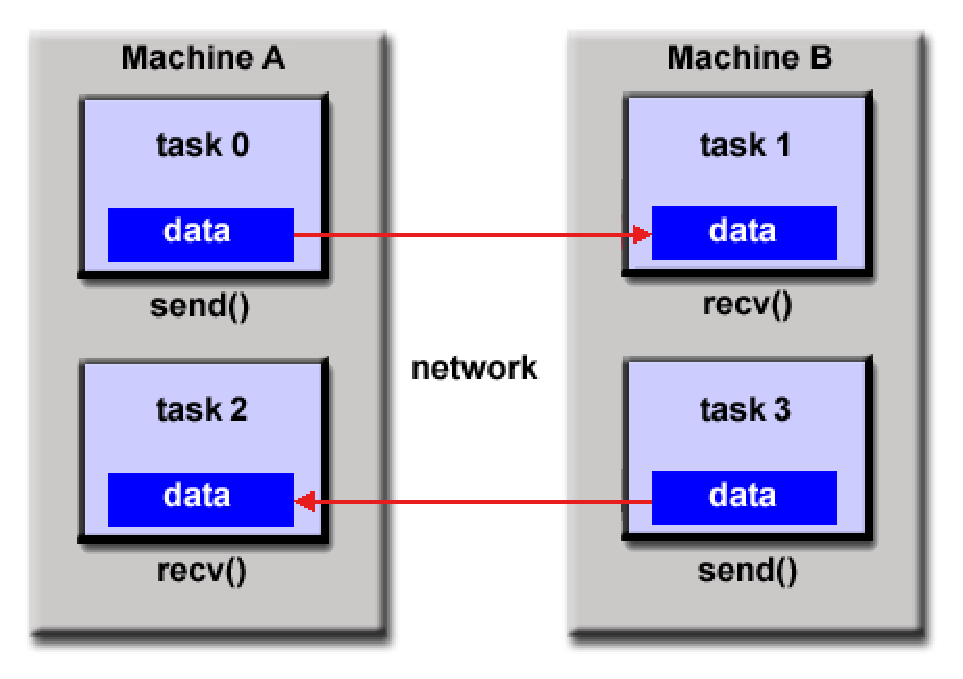
\includegraphics[width=0.8 \textwidth ]{OpenMP/pass_model.eps}
\end{center}
\small{
\caption[The message passing model]{
The message passing model can be implemented on the same machine or on several
machines connected in the network. Each task has his own data and shares the
intermediate results with messages across the network.
\label{Fig:Parallel:passModel}}}
\end{figure}

This design choice the author adopted was thus to develop a bare bones simulator
which is Thread safe and can be used with OpenMP.
The simulator Empass contains the following features:
\begin{itemize}
 \item world environment can have a circular or square geometry
 \item robotic agent and obstacle entities modeled as disks
 \item particle physic computation for elastic and non elastic collisions
 \item efficient distance calculation with sparse matrixes in Boost library
 \item logging data in CSV format
 \item support for Gnuplot for visualizing data
\end{itemize}
The main use of this simulator is to run parametric simulations
of the social system. For example in Figure \ref{Fig:Parallel:Empass}
there are N different configurations of the social system where
the black disks are the obstacles and the white disks are the agent.
Each configuration will run for $T_{sim}$ steps and is independent
from the others.

\begin{figure}[htbp]
\begin{center}
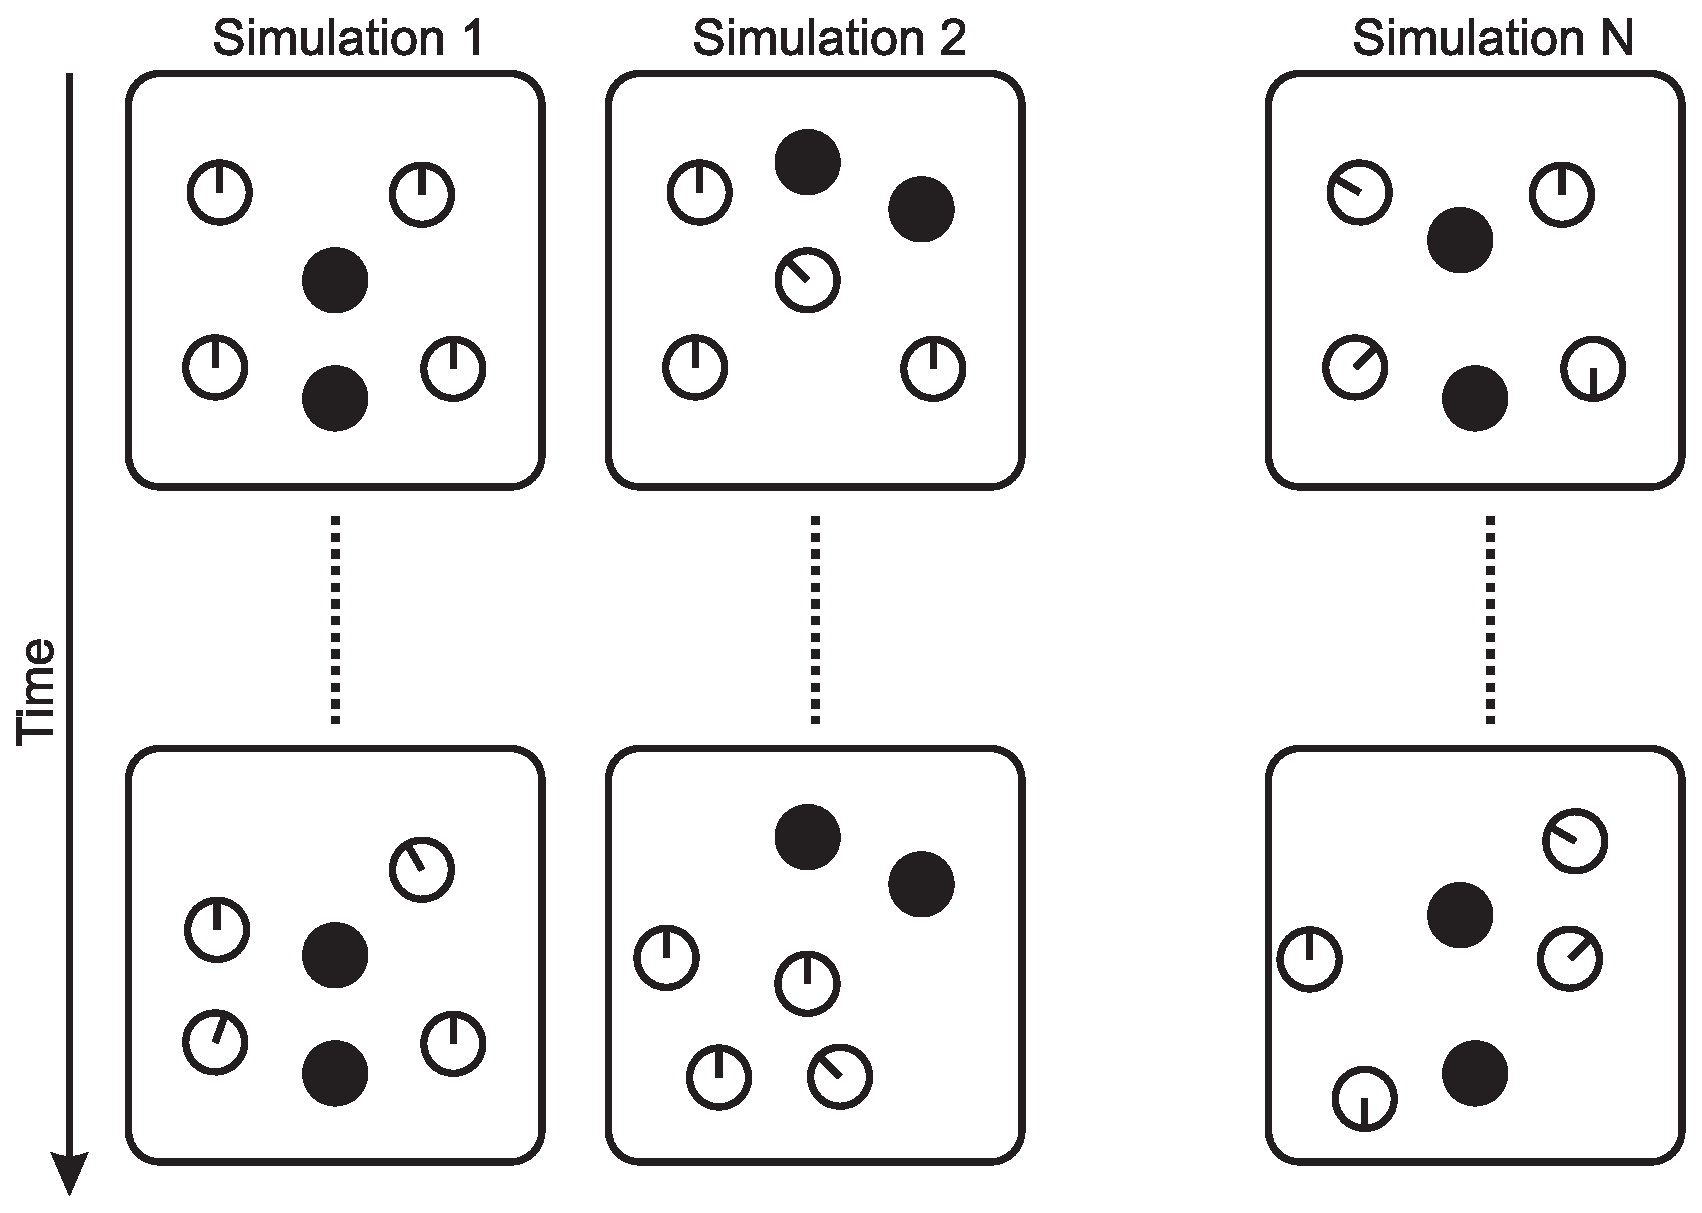
\includegraphics[width=0.8 \textwidth ]{OpenMP/FigureSimulator.eps}
\end{center}
\small{
\caption[Empass simulator]{
Graphical representation of a typical simulation with Empass.
There are N simulations which differs for the initial configuration of
the agents and obstacle location. Each simulation is independent from
the others and thus can be parallelised.
\label{Fig:Parallel:Empass}}}
\end{figure}

The following code is a sequential implementation for a typical simulation
run where there are 10 agents and 4 obstacles in a square world of 100 for
100 units.
There are a total of $Nsim=100$ different simulations that have to be run for
$T_{sim}=10000$ time steps.
Each configuration will generate different results because the initial conditions
are randomised.
\begin{lstlisting}
N=10;     // agents
M=4;     // obstacles
simtime=10000;  // simulation time

for(int conf=0;conf<Nsim;conf++)
{
    //create 100x100 unit square worlds
    world[conf]=World2DCartesian(100,100);
}

for(int conf=0;conf<Nsim;conf++)
{

    world[conf].run(N,M,simtime,false);

}
\end{lstlisting}

The previous code is the implementation of the same simulation code
but using the \textbf{parallel region construct} and the
\textbf{work sharing construct} as in Figure \ref{Fig:Parallel:fork}.

\begin{figure}[htbp]
\begin{center}
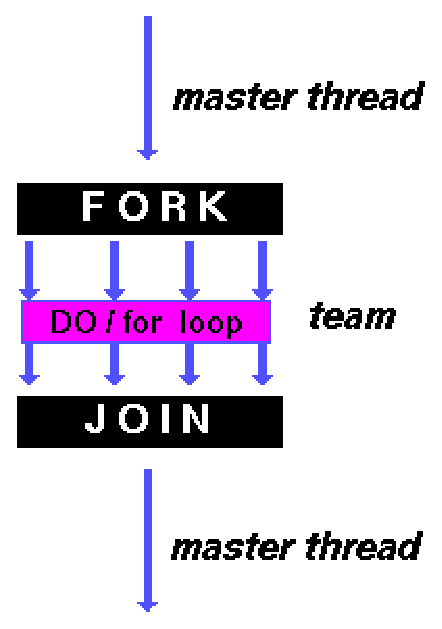
\includegraphics[width=0.3 \textwidth ]{OpenMP/work_share1.eps}
\end{center}
\small{
\caption[OpenMP fork loop]{
How OpenMP fork and join a while loop.
\label{Fig:Parallel:fork}}}
\end{figure}

\begin{lstlisting}
N=10;     // agents
M=4;     // obstacles
simtime=10000;  // simulation time
int chunk=10;
int conf=0;

for(int conf=0;conf<Nsim;conf++)
{
    //a 100x100 unit square world
    world[conf]=World2DCartesian(100,100);

}

#pragma omp parallel shared(N,M,simtime,world,chunk) private(conf)
{
    #pragma omp for schedule(dynamic,chunk) nowait
    for(conf=0;conf<Nsim;conf++)
    {
      world[conf].run(N,M,simtime,false);
    }
}
\end{lstlisting}
The tests were performed on two Linux machines, one with an Intel Core2 Quad CPU Q6600
at 2.40GHz with 4GB RAM DDRII memory and another one with Intel Core Duo  at 2.40 GHz with 2 GB RAM DDR memory.
The Table \ref{tab:Parallel:benchmark} shows how the execution time is drastically
reduced by a factor of 3.25, ideally one could achieve a factor of 4.0 because
there are virtually 4 CPU but this is not possible due to the actual hardware
implementation.
For $N_{sim}=10000$ the experimenter could easily have waited 1 minutes and 13 seconds
whereas with the parallel implementation only 35.63 seconds.
It is also interesting to note that there was not any significant difference in terms of performance
between the Intel Core Duo and the Intel Quad CPU.
\begin{table}[htbp]
\caption[Parallel Simulator performance]{
Table with some benchmarking measures}
\label{tab:Parallel:benchmark}
\begin{center}
\small{
\begin{tabular}{@{}c|ccc@{}}
\hline
Configuration & Processor & Sequential& OpenMP \\
\hline
$N_{sim}=1000$   & Intel Quad CPU     &  0m13.285s & 0m4.082s  \\
$N_{sim}=10000$  & Intel Quad CPU     &  1m13.178s & 0m35.637s \\
$N_{sim}=1000$   & Intel Core Duo CPU &  0m7.088s & 0m3.584s   \\
$N_{sim}=10000$  & Intel Core Duo CPU &  1m10.840s & 0m35.647s \\
\hline
\end{tabular}
}
\end{center}
\end{table}

This is only a very simple optimisation included in the simulator but there are
other possible optimisation strategies for the collision computation or
the communication protocol.
The next section describes a very important optimisation which was not implemented
for time constraints but is very important for future simulators.
\subsection{Pruning the parallel simulator}
Another optimisation that can be introduced is to ``prune'' the task execution.
In some occasions for a particular set of parameters a simulation can reach a
a looping stage where the agents are repeating their trajectories due to
an unfortunate positioning of the obstacles.
In this condition the simulation can be terminated because , the data produced
is of no use.
In Figure \ref{Fig:Parallel:pruneSim}, the simulation $X+1$ must be terminated
because the agent has incurred in a trajectory loop due to the obstacle configuration.
Simulation $X$ instead does not contain any loop condition.
\begin{figure}[htbp]
\begin{center}
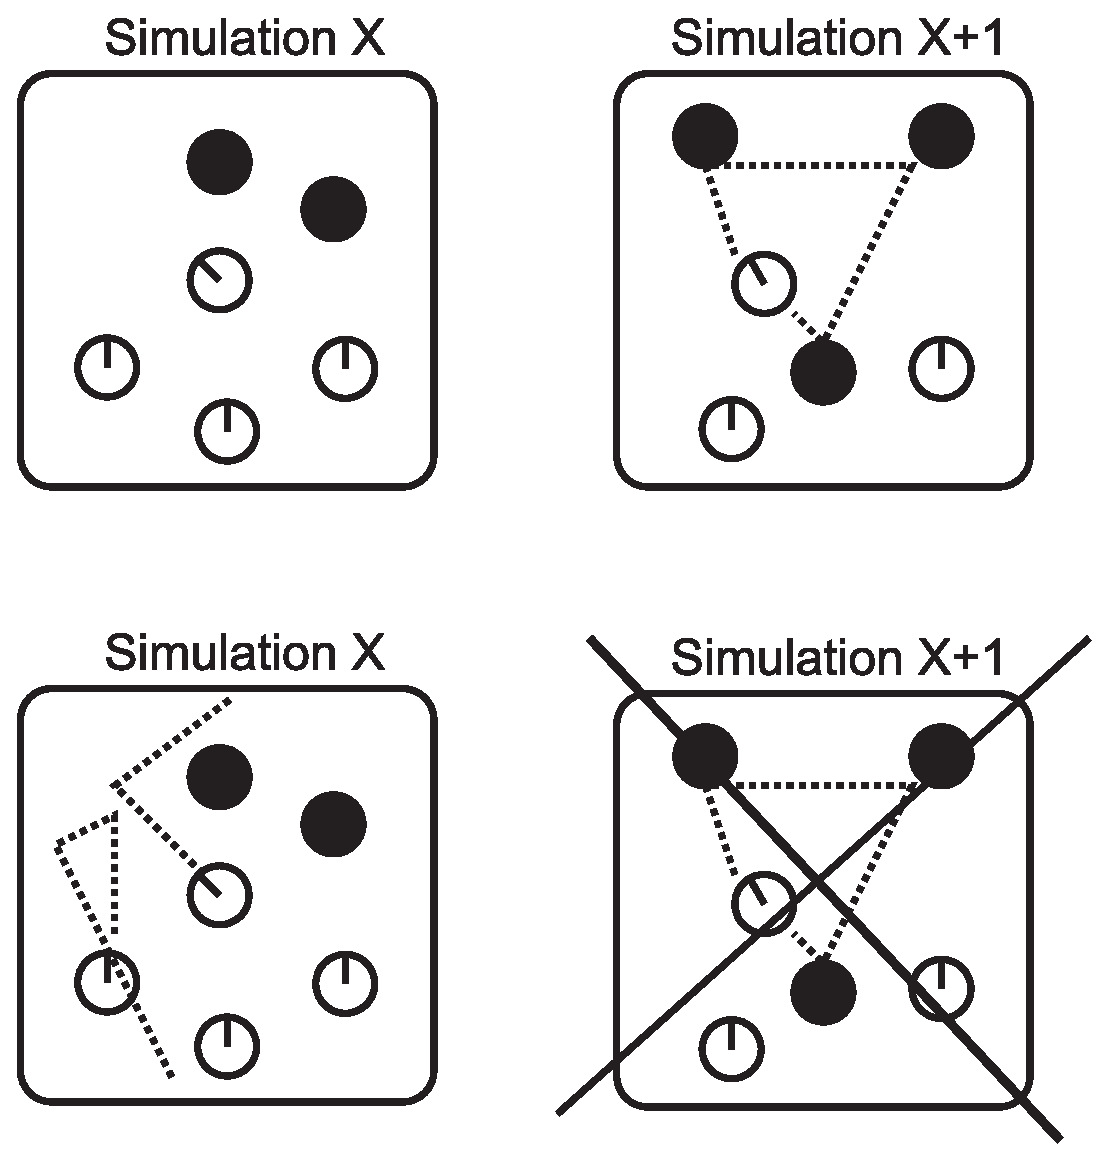
\includegraphics[width=0.5 \textwidth ]{OpenMP/FigureSimulatorLoop.eps}
\end{center}
\small{
\caption[Pruning parallel simulations]{
The agent in the simulator labelled with $X+1$ incurred in a trajectory loop,
and thus the simulation is stopped.
\label{Fig:Parallel:pruneSim}}}
\end{figure}
If the detection of the loop is shared between the simulation tasks this will
improve even more dramatically the performances by essentially removing
the tasks which are not useful.
This feature was not implemented as it required a more advanced inter communication
between tasks and is left as a future function.
There is also a novel approach that can be used to predict if an initial
configuration of agents will reach a loop condition and is described
in Chapter \ref{Conclusion:ModelCheck}.

\subsection{Discussion}
The importance of supporting the Thread model in computer simulation is becoming
of more importance within the consumer desktop industry.
Intel multi core technology is a clear example, the Core 2 Duo CPU was released
on July 2006 and the latest version Core i7 EE with 6 cores was release in January 2011.
This means that more and more researcher have access to multi core hardware
but do not have the tools to speed up their simulations.
There is also another interesting growing branch of optimisation based on the
use of the CUDA SDK based on the Nvidia GPU hardware.
For example, CUDA now accelerates AMBER, a molecular dynamics simulation program
 used by more than 60,000 researchers in academia and pharmaceutical companies
 worldwide to accelerate new drug discovery.
It seems that computing is evolving from "central processing" on the CPU
to "co-processing" on the CPU and GPU. To enable this new computing paradigm,
NVIDIA invented the CUDA parallel computing architecture that is now shipping in
GeForce, ION, Quadro, and Tesla GPUs, representing a significant installed
 base for application developers.
The company producing AMD and ATI hardware are also trying to catch up with 
this field but they are still behind a useful implementation.
This is certainly an interesting trend for future researchers as well as
videogame producers.

